% !TEX program = xelatex
\documentclass[12pt]{article}
\usepackage{iftex}
\ifPDFTeX
    \usepackage[T2A]{fontenc}
    \usepackage[utf8]{inputenc}
\else
    \usepackage{fontspec}
    \IfFontExistsTF{CMU Serif}
        {\setmainfont{CMU Serif}}
        {\IfFontExistsTF{Times New Roman}
            {\setmainfont{Times New Roman}}
            {\setmainfont{TeX Gyre Termes}}}
\fi
\usepackage[russian]{babel}
\usepackage{amsmath}
\usepackage{amssymb}
\usepackage{graphicx}
\usepackage{float}
\usepackage{array}
\usepackage{geometry}
\usepackage{hyperref}

\geometry{left=3cm, right=3cm, top=2cm, bottom=2cm}
\hypersetup{colorlinks=true, linkcolor=black, citecolor=black, urlcolor=black}
\sloppy

\begin{document}

\begin{titlepage}
    \centering
    {\large Московский физико-технический институт\\[0.3cm]
    Физтех-школа природоподобных, плазменных и ядерных технологий им. И.В. Курчатова\\[0.3cm]
    Кафедра моделирования ядерных процессов и технологий\par}

    \vspace{2.5cm}

    {\Large\bfseries Магистерская дипломная работа\par}

    \vspace{1.5cm}

    {\LARGE\bfseries Моделирование импульсного энерговвода в системе ТВЭЛ--вода и оценка предельных условий высокотемпературного разложения водяного пара\par}

    \vspace{2.5cm}

    \begin{flushright}
        \begin{tabular}{>{\raggedleft\arraybackslash}p{5cm}p{7cm}}
            Выполнил: & студент группы М07-405\\
            & Елесин Георгий Павлович\\[0.4cm]
            Направление: & 03.04.01 Прикладные математика и физика\\[0.4cm]
            Профиль: & Общая и прикладная физика\\[0.4cm]
            Специализация: & Суперкомпьютерное моделирование в прикладной физике\\[0.4cm]
            Научный руководитель: & Цибульский Виктор Филиппович\\
        \end{tabular}
    \end{flushright}

    \vfill

    {Москва, 2026}
\end{titlepage}

\tableofcontents
\newpage

\section{Введение}

Неэлектрические применения атомной энергии, включая высокотемпературное тепло и водородную энергетику, имеют смысл рассматривать только после локальной проверки физической реализуемости. Для системы ТВЭЛ--вода такой проверкой является не общий вопрос "можно ли получить водород", а более узкая расчетная задача: какая часть энергии, импульсно выделенной в топливе, за конечное время проходит через зазор и оболочку в воду или пар, где именно возникают высокие температуры и не наступает ли раньше повреждение топлива или оболочки.

В данной работе ТВЭЛ рассматривается как цилиндрическая тепловая система с топливом \(UO_2\), газовым зазором, металлической оболочкой и внешним водным или паровым слоем. На входе задан импульс линейной мощности \(P'(t)\). На выходе требуется не только максимальная температура топлива, но и причинная цепочка
\[
P'(t)\rightarrow T_f(r,t)\rightarrow T_c(r,t)\rightarrow q''_{cw}(t)
\rightarrow T_s(t),p_s(t),m_s(t)\rightarrow n_{H_2}^{\max}.
\]
Именно эта цепочка отделяет физически корректную постановку от некорректного утверждения, что высокий нагрев топлива автоматически означает высокотемпературный пар у поверхности оболочки.

Цель работы состоит в построении физико-математической модели импульсного энерговвода в системе ТВЭЛ--вода/пар и в оценке предельных условий, при которых возможен высокотемпературный нагрев водяного пара и ненулевой термолизный выход водорода. Объект исследования -- локальный участок системы "топливо--зазор--оболочка--вода/пар". Предмет исследования -- нестационарный радиальный теплоперенос, тепловая инерция топлива, сопротивление зазора, теплообмен на поверхности оболочки, фазовые переходы воды, перегрев пара и энергетические ограничения диссоциации \(H_2O\).

Главный исследовательский вопрос формулируется так: может ли локальный импульсный энерговвод в неразрушенный ТВЭЛ создать у оболочки и в прилегающем слое пара условия, достаточные для заметной термической диссоциации воды, раньше, чем система переходит в режим аварийного повреждения топлива или оболочки? В такой формулировке отрицательный ответ не является неудачей; он может быть основным научным результатом, если получен через проверяемые температурные, энергетические и материальные критерии.

В работе сознательно разводятся три разных механизма. Термическая диссоциация водяного пара является эндотермическим газофазным процессом и требует очень высоких температур, пониженного давления или специальных условий закалки продуктов. Пароциркониевая реакция является аварийным экзотермическим взаимодействием горячей оболочки с паром и не должна засчитываться как целевой термолиз. Кризис теплообмена и пленочное кипение являются теплогидравлическими режимами, которые могут привести к локальному перегреву и ухудшению теплоотвода, но сами по себе не являются полезной технологией производства \(H_2\) \cite{IAEATECDOC1578,TsutsumiWaterSplitting,LOCAOxidation}.

\section{Научная постановка и рамка руководителя}

Постановка работы строится в логике, характерной для научной школы В.Ф.~Цибульского: детальный расчет локальной физики должен завершаться системным критерием применимости. В его работах по реакторной физике и развитию ядерной энергетики локальные величины -- температурное поле, коэффициенты реактивности, выгорание, состав топлива -- не остаются сами по себе, а переводятся в вывод о ресурсности, безопасности, приемлемости топливного цикла и эволюционной реализуемости энергетической схемы \cite{CibulskyEnergySecurity2006,DESAE2008,CibulskyTempCoeff2014,CibulskyStrategy2022}.

Для настоящей работы это означает следующую структуру аргумента:
\[
\begin{gathered}
\text{локальная физика ТВЭЛа}\\
\downarrow\\
\text{редуцированная модель передачи энергии к воде}\\
\downarrow\\
\text{энергетический и материальный баланс}\\
\downarrow\\
\text{критерий технической реализуемости}\\
\downarrow\\
\text{системный вывод о применимости ядерного источника}.
\end{gathered}
\]
Водородная тематика при этом не вводится как самостоятельное обещание технологии. Она используется как жесткая выходная метрика: если расчет показывает, что энергия не успевает попасть в паровую область до плавления топлива, деградации оболочки или перехода в severe-accident режим, то схема не проходит физический критерий.

Предыдущий задел по доплеровской памяти не является центральной темой новой редакции. Он остается полезным как диагностический пример того, что история энерговыделения в топливе имеет запаздывающие выходы. Однако основной канал данной работы -- не реактивностное ядро \(K_D\), а тепловой выход из топлива к воде:
\[
Q_{fw}(t)=\int_0^t H_{fw}(t-s)P'(s)\,ds.
\]
Это выражение допускается только как редуцированная форма полной радиальной тепловой задачи: ядро \(H_{fw}\) не заменяет физику топлива, зазора, оболочки и кипения, а сжимает ее в причинный отклик для заданной геометрии и режима.

\section{Физическая модель системы ТВЭЛ--вода/пар}

Рассматривается локальный осесимметричный участок твэла длиной \(L=1\,\mathrm{m}\). Топливная таблетка занимает область \(0<r<R_f\), газовый зазор задается эффективным тепловым сопротивлением, оболочка занимает область \(R_g<r<R_o\), а снаружи находится вода, насыщенная смесь или пар. Объемный источник в топливе для линейной мощности \(P'(t)\) записывается как
\[
q'''(t)=\frac{P'(t)}{\pi R_f^2}.
\]

Топливо \(UO_2\) описывается нестационарной теплопроводностью в цилиндре:
\[
\rho_f c_f(T_f)\frac{\partial T_f}{\partial t}
=
\frac{1}{r}\frac{\partial}{\partial r}
\left(k_f(T_f)r\frac{\partial T_f}{\partial r}\right)
+q'''(t),\qquad 0<r<R_f.
\]
На оси выполняется условие симметрии
\[
\left.\frac{\partial T_f}{\partial r}\right|_{r=0}=0.
\]
Топливо является главным аккумулятором энергии короткого импульса: из-за малой температуропроводности \(UO_2\) максимум температуры сначала возникает внутри таблетки, а не в воде \cite{IAEATHPH2007,IAEATECDOC1496}.

Газовый зазор в базовой модели не выделяется как отдельная объемная область, а задается законом теплопередачи
\[
q''_g(t)=h_g(t)\left(T_{f,s}(t)-T_{c,i}(t)\right),
\]
где \(T_{f,s}\) -- температура поверхности топлива, \(T_{c,i}\) -- температура внутренней поверхности оболочки, \(h_g\) -- эффективная проводимость зазора. В развитой модели \(h_g\) должен зависеть от температуры, состава газа, давления и закрытия зазора.

Оболочка описывается собственной радиальной теплопроводностью:
\[
\rho_c c_c(T_c)\frac{\partial T_c}{\partial t}
=
\frac{1}{r}\frac{\partial}{\partial r}
\left(k_c(T_c)r\frac{\partial T_c}{\partial r}\right),
\qquad R_g<r<R_o.
\]
Сопряжение с топливом и зазором задается потоком \(q''_g\), а на внешней поверхности:
\[
-k_c\left.\frac{\partial T_c}{\partial r}\right|_{R_o}=q''_{cw}(t),
\qquad
q''_{cw}=\mathcal{Q}(T_s,T_\infty,p,G,\chi).
\]
Функция \(\mathcal{Q}\) должна выбираться по режиму теплообмена: однофазная конвекция, пузырьковое кипение, кризис теплообмена, переходное кипение или пленочное кипение. Одна постоянная теплоотдачи \(h\) не является достаточным замыканием для предельного режима \cite{IAEATECDOC1578}.

\begin{figure}[H]
    \centering
    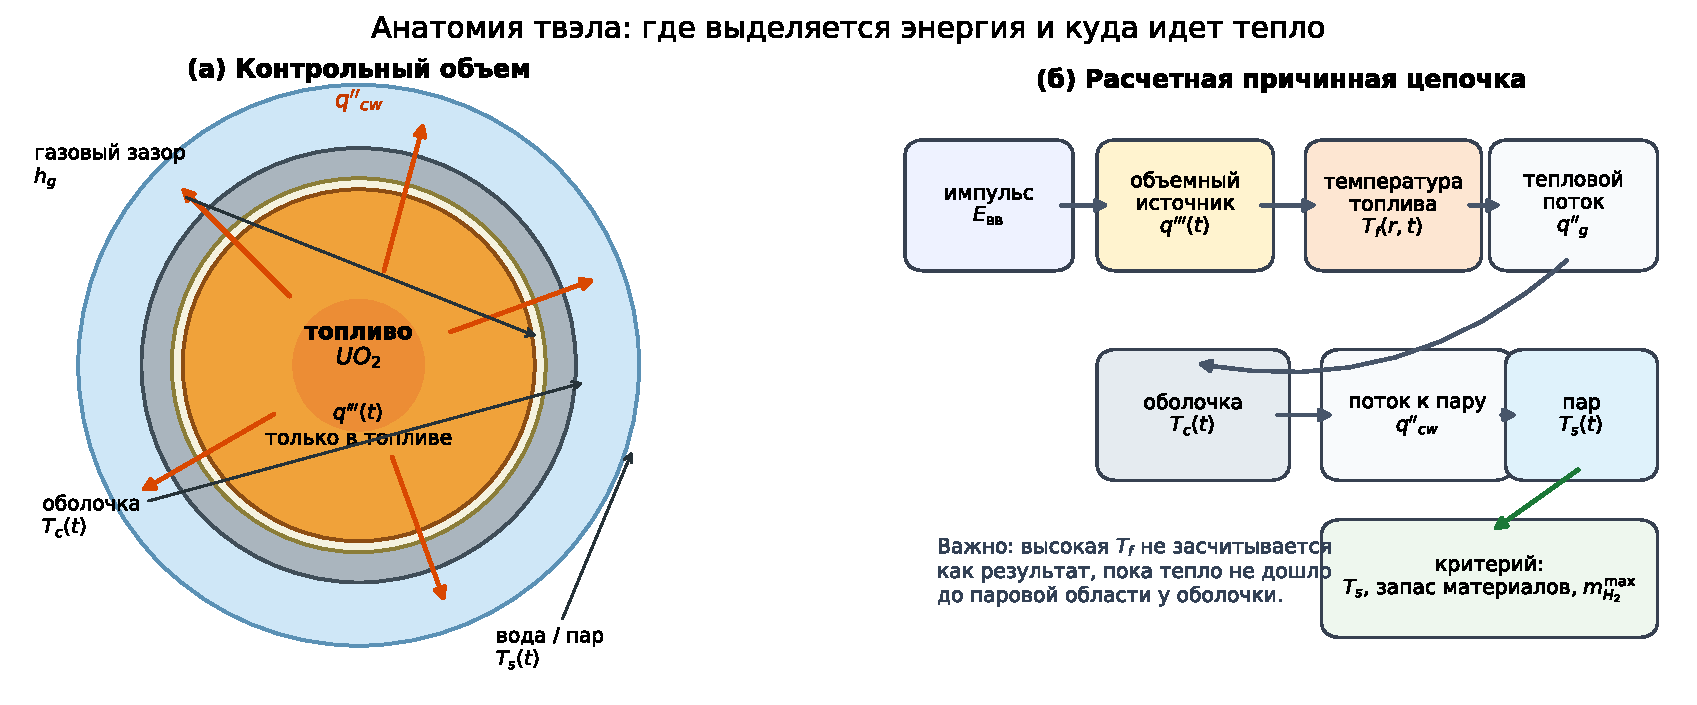
\includegraphics[width=\textwidth]{figures/fig7_fuel_pin_anatomy.pdf}
    \caption{Расчетная область: энерговыделение возникает в топливе \(UO_2\), затем энергия проходит через газовый зазор и оболочку к воде или пару. Высокая температура топлива сама по себе не означает высокую температуру паровой области.}
    \label{fig:fuelPinAnatomyTheory}
\end{figure}

\section{Характерные времена и причинная передача энергии}

Ключевой физический параметр задачи -- не только максимум температуры, но и иерархия времен. Вводится число краткости импульса
\[
\Pi_\tau=\frac{\tau_p}{\tau_f}.
\]
Если \(\Pi_\tau\ll1\), импульс почти адиабатичен для радиальной теплопроводности топлива. Тогда большая часть внесенной энергии сначала остается в \(UO_2\), а вода видит лишь задержанный тепловой выход через топливо, зазор и оболочку.

Для модельного твэла с \(R_f=4\,\mathrm{mm}\), \(\delta_g=80\,\mathrm{\mu m}\), \(\delta_c=0.65\,\mathrm{mm}\) и характерными свойствами \(UO_2\) получается \(\alpha_f\approx1.3\cdot10^{-6}\,\mathrm{m^2/s}\). Масштаб \(R_f^2/\alpha_f\) имеет порядок \(12\,\mathrm{s}\), а первая радиальная мода -- порядка секунд. Для циркониевой оболочки \(\alpha_c\sim(8-10)\cdot10^{-6}\,\mathrm{m^2/s}\), поэтому диффузионное время через оболочку порядка \(4\cdot10^{-2}\,\mathrm{s}\). Через открытый газовый зазор при \(h_g\sim(5-20)\cdot10^3\,\mathrm{W/(m^2K)}\) возникает дополнительная задержка порядка \(0.07-0.3\,\mathrm{s}\).

\begin{figure}[H]
    \centering
    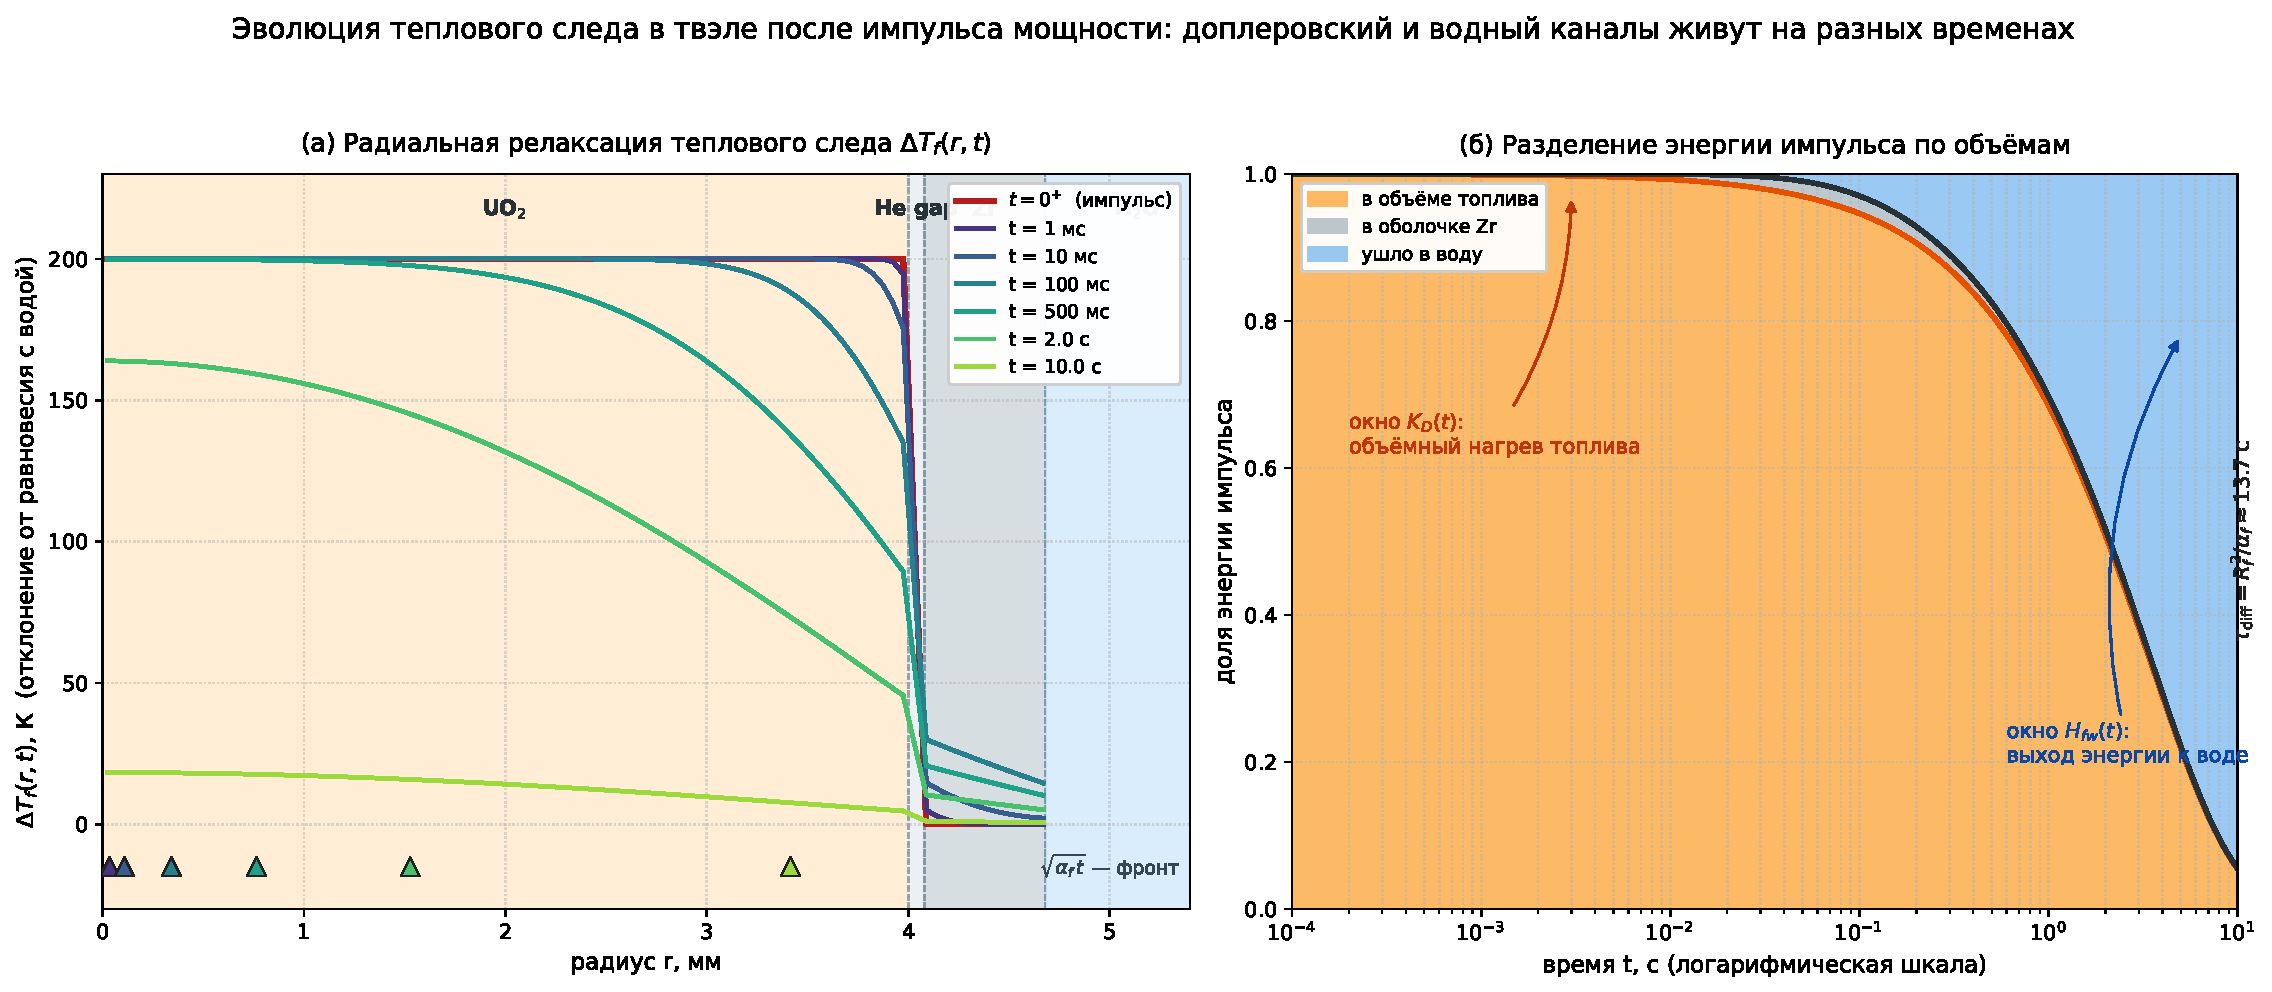
\includegraphics[width=\textwidth]{figures/fig14_thermal_radial_relaxation.pdf}
    \caption{Радиальная тепловая релаксация твэла после короткого импульса мощности. В первые миллисекунды энергия остается главным образом в топливе; заметный выход к воде формируется на более длинном тепловом масштабе и может быть описан редуцированным ядром \(H_{fw}\).}
    \label{fig:thermalRadialRelaxation}
\end{figure}

Для водной стороны важны два разных факта. Тонкий слой у стенки может нагреваться быстро по масштабу \(\tau_{w,\delta}\sim\delta^2/\alpha_w\), но это не отменяет затрат на кипение, испарение и перегрев. Поэтому расчет обязан указывать не только температуру, но и массу воды или пара, длительность существования высокотемпературной области и энергию, дошедшую до этой области:
\[
\eta_{fw}(t_{\mathrm{obs}})=
\frac{Q_w(t_{\mathrm{obs}})}{E_{\mathrm{imp}}}.
\]

\section{Энергетический баланс воды, пара и \texorpdfstring{\(H_2\)}{H2}}

Интегральный баланс по единице длины записывается как
\[
E_{\mathrm{imp}}(t)=\int_0^tP'(\tau)d\tau,
\]
\[
E_{\mathrm{imp}}
=
\Delta U_f+\Delta U_c
+Q_{w,\mathrm{sens}}+Q_{\mathrm{evap}}+Q_{s,\mathrm{sup}}
+Q_{\mathrm{diss}}+Q_{\mathrm{ox}}+Q_{\mathrm{loss}}.
\]
В целевом термолизном режиме член \(Q_{\mathrm{ox}}\), связанный с окислением оболочки, должен быть мал. Если водород получается главным образом из пароциркониевой реакции, физический смысл результата меняется: это уже аварийный механизм образования \(H_2\), а не высокотемпературное разложение водяного пара.

Для воды и пара используется энтальпийное разбиение. До кипения:
\[
Q_{w,\mathrm{sens}}=
m_l\left[h_f(T_{\mathrm{sat}},p)-h_l(T_0,p)\right].
\]
На стадии испарения:
\[
Q_{\mathrm{evap}}=m_{\mathrm{ev}}h_{fg}(p).
\]
На стадии перегрева пара:
\[
Q_{s,\mathrm{sup}}=
m_v\left[h_s(T_s,p)-h_g(T_{\mathrm{sat}},p)\right].
\]
Свойства воды и пара должны задаваться по IAPWS-IF97 или сопоставимым таблицам, а не по произвольной постоянной теплоемкости во всем диапазоне \cite{IAPWSIF97,AlexandrovGrigoriev}.

После вычитания затрат на нагрев, испарение и перегрев вводится энергия, потенциально доступная для диссоциации:
\[
Q_{\mathrm{diss}}^{\max}=
\max\left\{0,\,
Q_{w\to s}
-Q_{\mathrm{heat+boil+superheat}}^{\min}(T^*_{\mathrm{diss}},p)
\right\}.
\]
Абсолютный молярный предел:
\[
n_{H_2}^{\max}=
\frac{Q_{\mathrm{diss}}^{\max}}{\Delta H_{\mathrm{diss}}},
\qquad
\Delta H_{\mathrm{diss}}\approx241.93\,\mathrm{kJ/mol}.
\]
Эта величина является верхней границей, а не прогнозом. Реалистическая оценка должна содержать хотя бы равновесный и квенч-факторы:
\[
n_{H_2}^{\mathrm{real}}\le
\eta_{\mathrm{eq}}(T,p)\eta_q n_{H_2}^{\max},
\qquad 0\le\eta_{\mathrm{eq}},\eta_q\le1.
\]
Прямой термолиз становится заметным только при очень высоких температурах; при \(3000\,\mathrm{K}\) и \(1\,\mathrm{atm}\) равновесная диссоциация водяного пара все еще далека от полной, а повышение давления дополнительно сдвигает равновесие к воде \cite{TsutsumiWaterSplitting}.

Критерии реализуемости собираются в логическое условие
\[
\mathcal C_{\mathrm{target}}=
(\Theta_{\mathrm{diss}}>1)
\land(M_c>0)
\land(M_f>0)
\land(\text{нет FCI})
\land(Q_{\mathrm{ox}}\ll Q_{\mathrm{diss}}),
\]
где
\[
\Theta_{\mathrm{diss}}=\frac{T_{s,\max}}{T^*_{\mathrm{diss}}(p)},
\qquad
M_f=T_{m,f}-T_{f,\max},
\qquad
M_c=T_{c,\lim}-T_{c,\max}.
\]
Для \(UO_2\) температура \(3000^\circ\mathrm{C}\approx3273\,\mathrm{K}\) уже выше рекомендованной температуры плавления порядка \(3120\pm30\,\mathrm{K}\). Для циркониевой оболочки такая температура тем более невозможна как твердофазный режим: характерная температура плавления циркониевых сплавов существенно ниже. Поэтому всякий расчет с \(T_f>T_{m,f}\) или \(T_c>T_{c,\lim}\) должен интерпретироваться как переход к аварийной области, а не как достижение целевого термолизного режима \cite{IAEATECDOC1496,IAEATECDOC1578,LOCAOxidation,OECDFCI}.

\section{Расчетная реализация и синхронизированные рисунки}

Расчетная часть работы строится в два уровня. Базовым уровнем для дальнейшей полной постановки остается GeN-Foam: он должен отвечать за нестационарное энерговыделение, радиальный теплоперенос в модели \texttt{nuclearFuelPin}, теплообмен с теплоносителем и выгрузку временных рядов \(T_f(r,t)\), \(T_c(t)\), \(q''_{cw}(t)\), \(Q_w(t)\) \cite{GeNFoam2015,foamForNuclear2026}. Химический блок не заменяет теплогидравлику: он получает уже рассчитанное состояние пара \(T_s(t),p_s(t),m_s(t)\) и дает только равновесную или энергетически ограниченную верхнюю оценку \(H_2\) \cite{CanteraEquilibrium2026}.

В текущей редакции для проверки всей цепочки используется компактный notebook-pipeline \texttt{01\_tvel\_water\_pipeline.ipynb}. Его роль ограничена отладкой расчетной логики: задать один метр твэла, внести импульс энергии в топливо, провести энергию через зазор и оболочку, нагреть малую приповерхностную паровую прослойку и проверить критерии \(T_s>T^*_{\mathrm{diss}}\), \(M_f>0\), \(M_c>0\). Этот Python-расчет не является второй физической моделью твэла для финального вывода; он нужен как воспроизводимый предельный экран до переноса сценария в GeN-Foam.

Численная схема notebook-pipeline является явной конечно-объемной аппроксимацией радиальной задачи. Для ячейки \(i\) с объемом \(V_i\) и теплоемкостью \((\rho c)_i\) используется баланс
\[
(\rho c)_iV_i\frac{T_i^{n+1}-T_i^n}{\Delta t}
=
F_{i-1/2}^n-F_{i+1/2}^n+S_i^n,
\]
где внутренние потоки считаются по теплопроводности, поток через газовый зазор задается \(h_g(T_{f,s}-T_{c,i})\), а поток с наружной поверхности оболочки в паровую прослойку задается \(h_s(T_{c,o}-T_s)\). Накопленная энергия паровой прослойки переводится в температуру и верхнюю оценку диссоциации по формулам раздела энергетического баланса.

Чтобы рисунки в дипломе не расходились с notebook-расчетом, они подключаются через генерируемый фрагмент \texttt{figures/pipeline\_report.tex}. Команда \texttt{make pipeline-figures} запускает \texttt{scripts/export\_pipeline\_figures.py}, пересчитывает те же сценарии, что и ноутбук, обновляет файлы \texttt{figures/pipeline\_*.png} и затем пересоздает LaTeX-фрагмент с рисунками и таблицей.

\subsection{Версия 1 пайплайна: \texorpdfstring{\(UO_2\)--Zircaloy}{UO2--Zircaloy}}

Эта версия фиксирует штатную пару \(UO_2\)--Zircaloy и использует тепловой ряд GeN-Foam; идентификатор расчета -- \texttt{zircaloy-v1}. Рассматривается один метр твэла с радиусом топлива \(R_f=4.00\,\mathrm{мм}\), зазором \(80\,\mu\mathrm{m}\), оболочкой толщиной \(0.60\,\mathrm{мм}\) и приповерхностным слоем воды толщиной \(\delta_w=100\,\mu\mathrm{m}\) при \(p_w=15.5\,\mathrm{МПа}\). Входной импульс равен \(E_{\mathrm{вв}}=250\,\mathrm{кДж/м}\), а для оболочки используется допустимый предел \(T_{\mathrm{lim},c}=1477\,\mathrm{K}\), а не температура плавления.

Масса воды у оболочки считается из кольцевого контрольного объема:
\[
m_w'=\rho_l \pi\left[(R_c+\delta_w)^2-R_c^2\right].
\]
Для выбранных параметров \(m_w'\approx1.932\,\mathrm{г/м}\). Сначала этот слой испаряется, затем сухой пар может перегреваться. В расчет введено физическое ограничение \(T_s(t)\le T_c(t)\): пар, нагреваемый только через оболочку, не может быть горячее наружной стенки.

\begin{figure}[H]
    \centering
    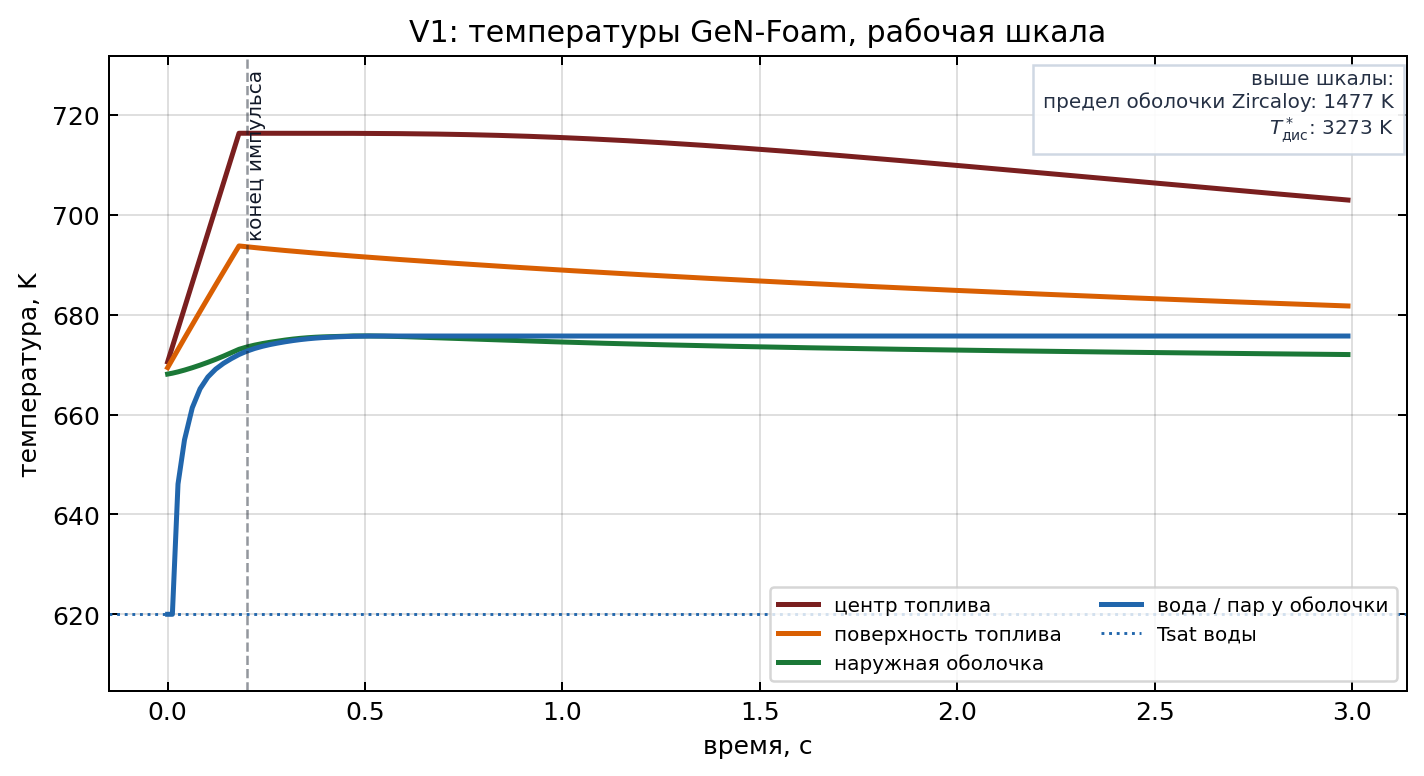
\includegraphics[width=0.82\textwidth]{figures/pipeline_temperature_history.png}
    \caption{Версия 1: история температур \(UO_2\)--Zircaloy при \(E_{\mathrm{вв}}=250\,\mathrm{кДж/м}\). Водно-паровой слой не достигает порога \(T^*_{\mathrm{дис}}=3273\,\mathrm{K}\), а оболочка остается ниже принятого температурного предела.}
    \label{fig:pipelineTemperatureHistory}
\end{figure}

Энергетический график нормирован на полную энергию импульса:
\[
\varepsilon_j(t)=\frac{E_j(t)}{E_{\mathrm{вв}}},
\qquad
j\in\{f,c,s\}.
\]
Здесь \(E_s\) означает энергию в локальном водно-паровом объеме около оболочки после нагрева, испарения и возможного перегрева. В версии 1 водно-паровая область получает \(\varepsilon_s\approx0.962\,\%\) импульса после ограничения температурой стенки. Теплоемкость сухого пара в этом объеме равна \(C_s'\approx5.023\,\mathrm{Дж/(К\cdot м)}\), но до перегрева надо также покрыть скрытую теплоту испарения.

\begin{figure}[H]
    \centering
    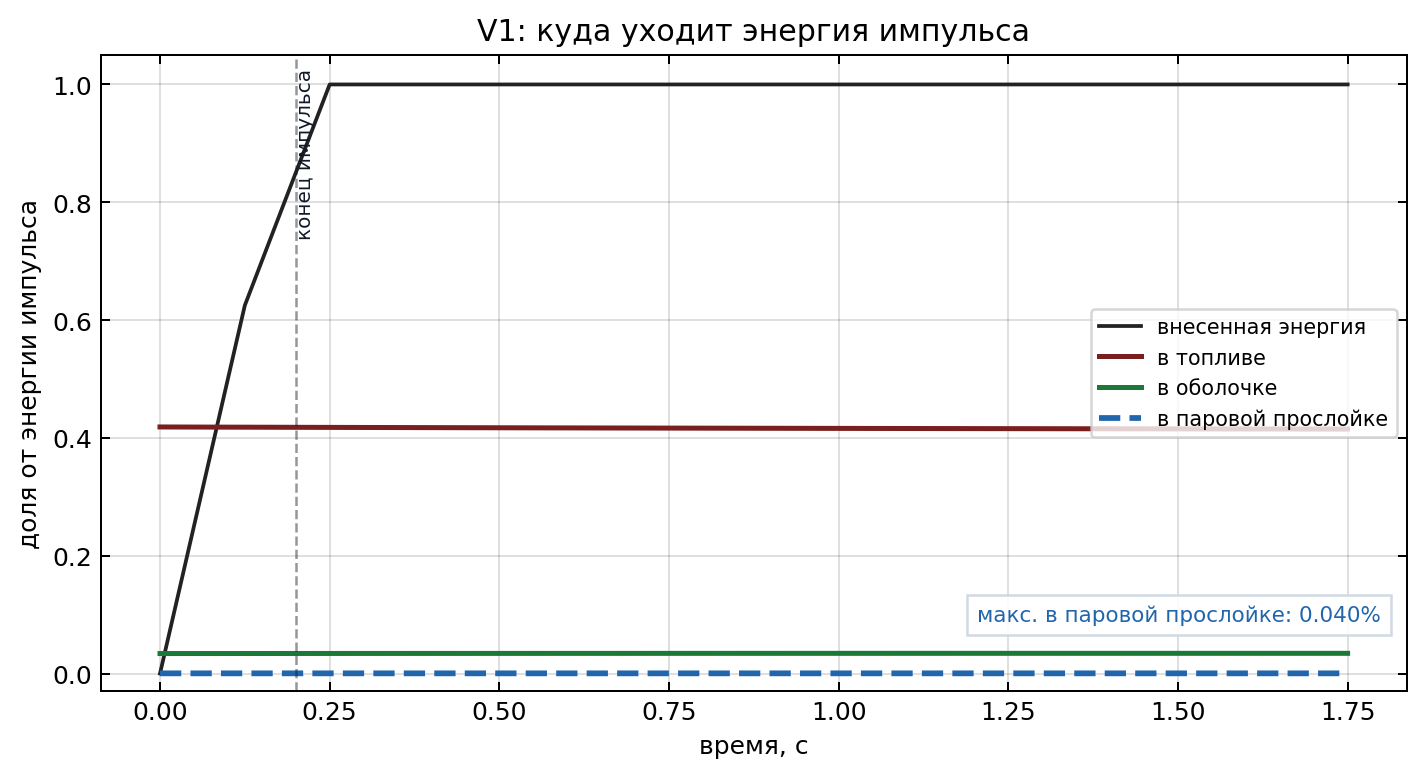
\includegraphics[width=0.82\textwidth]{figures/pipeline_energy_balance.png}
    \caption{Доли энергии импульса, накопленные в топливе, оболочке и водно-паровом слое. Основная часть энергии остается в твердой части твэла или не попадает в локальный водный объем при выбранном ограничении стенкой.}
    \label{fig:pipelineEnergyBalance}
\end{figure}

Малую величину \(\varepsilon_s\) удобно разложить как энергетическую воронку. В строке «топливо и газовый зазор» показана энергия, которая к моменту \(t=3.0\,\mathrm{s}\) еще не дошла до оболочки по выгруженному ряду GeN-Foam. В строке «оболочка» показана энергия, которая уже прошла через зазор, но осталась в металле оболочки и не была передана паровой прослойке.

\begin{table}[H]
    \centering
    \caption{Энергетическая воронка версии 1 к концу расчета. Величины нормированы на \(E_{\mathrm{вв}}=250\,\mathrm{кДж/м}\).}
    \label{tab:pipelineEnergyFunnel}
    \small
    \resizebox{\textwidth}{!}{%
    \begin{tabular}{@{}p{4.2cm}rrrrr@{}}
    \hline
    Звено & Накоплено или не прошло, кДж/м & от \(E_{\mathrm{вв}}\), \% & от входа звена, \% & Прошло дальше, кДж/м & от \(E_{\mathrm{вв}}\), \% \\
    \hline
    Топливо и газовый зазор & 1.86 & 0.744 & 0.744 & 2.53 & 1.01 \\
    Оболочка & 0.13 & 0.052 & 5.10 & 2.40 & 0.962 \\
    \hline
    \end{tabular}
    }
\end{table}

Итоговая энергия в водно-паровом слое составляет \(E_s\approx2.405\,\mathrm{кДж/м}\), или \(0.962\,\%\) от импульса. До последнего расчетного момента с положительным запасом оболочки эта величина составляет \(E_s\approx2.405\,\mathrm{кДж/м}\), или \(0.962\,\%\). Главный ограничитель здесь не полная энергия импульса, а температура наружной оболочки: при \(T_c\ll T^*_{\mathrm{дис}}\) перегретый пар также остается далеко ниже порога диссоциации.

Равновесная химия считается в Cantera по состоянию пара из теплового ряда:
\[
T_s(t),\quad p_s(t),\quad X_0=\{H_2O:1\},
\qquad
m_{H_2}^{eq}=n_{H_2}^{eq}M_{H_2}.
\]
До выхода топлива и оболочки за принятые пределы водно-паровой слой успевает нагреться до \(T_s\approx676\,\mathrm{K}\). Полный расчетный максимум оболочки дает запас \(M_{\mathrm{об}}=T_{\mathrm{lim},c}-T_c^{\max}\approx801\,\mathrm{K}\). Топливо в этой точке еще не является первым ограничением, поскольку \(M_f\approx2404\,\mathrm{K}\).

\begin{table}[H]
    \centering
    \caption{Сводка версии 1: входной импульс и три основных выхода для \(UO_2\)--Zircaloy.}
    \label{tab:pipelineScenarioReport}
    \small
    \resizebox{\textwidth}{!}{%
    \begin{tabular}{@{}p{4.0cm}rp{2.2cm}p{2.4cm}p{2.2cm}p{5.4cm}@{}}
    \hline
    Сценарий & \(E_{\mathrm{вв}}\), кДж/м & \(T_{s,\max}^{M>0}\), K & \(M_{\mathrm{об}}\), K & \(m_{H_2}^{eq}\), г/м & Вывод \\
    \hline
    \(UO_2\)--Zircaloy, версия 1 & 250 & 676 & 801 & \(\ensuremath{7.61\cdot10^{-13}}\) & пределы топлива и оболочки не нарушены, но целевое температурное окно не достигнуто \\
    \hline
    \end{tabular}
    }
\end{table}

Итог версии 1 является отрицательным по термохимическому критерию: в принятом тепловом ряду топливо и оболочка остаются ниже своих пределов, но водно-паровой слой не выходит к выбранному порогу \(T^*_{\mathrm{дис}}\). Для принятого порога \(T^*_{\mathrm{дис}}\) температурный запас пара до нарушения пределов равен \(\Delta T_{\mathrm{зап}}\approx-2597\,\mathrm{K}\), а запас оболочки в полном расчете равен \(M_{\mathrm{об}}\approx801\,\mathrm{K}\).


\section{Выводы по контрольной постановке}

Базовый сценарий \(UO_2\)--Zircaloy при импульсе \(250\,\mathrm{kJ/m}\), паровой прослойке \(100\,\mu\mathrm{m}\) и давлении \(15.5\,\mathrm{MPa}\) не достигает химического окна термолиза. Температура прослойки в расчете поднимается только до порядка \(2.0\cdot10^3\,\mathrm{K}\), тогда как выбранный порог \(T^*_{\mathrm{diss}}\) равен \(3273\,\mathrm{K}\). При этом запас по оболочке уже мал, потому что предельная температура циркониевого сплава существенно ниже требуемого термолизного уровня.

Контрфактический расчет с высокотемпературной парой материалов \(HfC\)--W показывает другой смысл критерия. Даже когда температурное окно достигается без плавления материалов в этой грубой тепловой постановке, энергетически ограниченный верхний выход водорода остается порядка \(10^{-4}\,\mathrm{g/m}\). Это не технологический результат, а проверка масштаба: прямой высокотемпературный термолиз около твэла требует не только высокой температуры, но и достаточной массы пара, времени существования горячего слоя, квенча продуктов и сохранения конструкционной целостности.

Следовательно, основной научный вывод текущей редакции отрицателен и проверяем: для штатной пары \(UO_2\)--Zircaloy целевой термолизный режим не возникает до приближения к материальным ограничениям оболочки. Дальнейшие расчеты должны уточнять не сам факт высокой температуры топлива, а карту режимов в координатах \(E_{\mathrm{imp}},\tau_p,h_g,h_s,\delta_s,p\): где энергия остается в топливе, где перегревается оболочка, где начинается аварийная пароциркониевая область и существует ли вообще непустая область \(\mathcal C_{\mathrm{target}}=1\).

\newpage
\section{Список литературы}
\begin{thebibliography}{30}

\bibitem{CibulskyEnergySecurity2006}
Пономарев-Степной Н. Н., Цибульский В. Ф.
Атомная энергия и энергетическая безопасность.
\textit{Атомная энергия}, т. 101, вып. 4, с. 247--254, 2006.

\bibitem{DESAE2008}
Андрианова Е. А., Давиденко В. Д., Цибульский В. Ф.
Программа DESAE для системных исследований перспектив развития ядерной энергетики.
\textit{Атомная энергия}, т. 105, вып. 6, с. 303--306, 2008.

\bibitem{CibulskyTempCoeff2014}
Климов А. Д., Давиденко В. Д., Цибульский В. Ф. и др.
Температурный коэффициент реактивности ВВЭР-1000.
\textit{Атомная энергия}, 2014.

\bibitem{CibulskyStrategy2022}
Велихов Е. П. и др.
Возможности и перспективы крупномасштабной ядерной энергетики.
\textit{Вопросы атомной науки и техники. Серия: Физика ядерных реакторов}, № 2, 2022.

\bibitem{IAEATHPH2007}
Kirillov P. L. et al.
\textit{Thermophysical Properties of Materials for Nuclear Engineering: A Tutorial and Collection of Data}.
IAEA, 2007.

\bibitem{IAEATECDOC1496}
International Atomic Energy Agency.
\textit{Thermophysical Properties Database of Materials for Light Water Reactors and Heavy Water Reactors}.
IAEA-TECDOC-1496, 2006.

\bibitem{IAEATECDOC1578}
International Atomic Energy Agency.
\textit{Computational Analysis of the Behaviour of Nuclear Fuel under Accident Conditions}.
IAEA-TECDOC-1578, 2008.

\bibitem{LOCAOxidation}
International Atomic Energy Agency and related LOCA criteria reports.
\textit{High-temperature oxidation and post-quench ductility limits for zirconium alloy cladding}.

\bibitem{IAPWSIF97}
International Association for the Properties of Water and Steam.
\textit{Revised Release on the IAPWS Industrial Formulation 1997 for the Thermodynamic Properties of Water and Steam}.

\bibitem{AlexandrovGrigoriev}
Александров А. А., Григорьев Б. А.
\textit{Таблицы теплофизических свойств воды и водяного пара}.

\bibitem{TsutsumiWaterSplitting}
Tsutsumi A.
\textit{Thermodynamics of Water Splitting}.
Encyclopedia of Life Support Systems.

\bibitem{OECDFCI}
OECD Nuclear Energy Agency.
\textit{Fuel-coolant interaction and severe accident phenomenology reports}.

\bibitem{NRCFeedback2012}
U.S. Nuclear Regulatory Commission.
\textit{Reactor Concepts Manual: Reactor Theory and Feedback Effects}.
NRC Technical Training Center, 2012.
\url{https://www.nrc.gov/reading-rm/basic-ref/students/reactors.html}

\bibitem{DOEGeneralTechnicalBase2013}
U.S. Department of Energy.
\textit{Nuclear Physics and Reactor Theory. DOE Fundamentals Handbook}.
DOE-HDBK-1019/1-93, 2013.
\url{https://www.standards.doe.gov/standards-documents/1000/1019-bhdbk-1993-v1}

\bibitem{DuderstadtHamilton1976}
Duderstadt J. J., Hamilton L. J.
\textit{Nuclear Reactor Analysis}.
John Wiley \& Sons, 1976.

\bibitem{GeNFoam2015}
Fiorina C., Clifford I., Aufiero M., Mikityuk K.
GeN-Foam: a novel OpenFOAM based multi-physics solver for 2D/3D transient analysis of nuclear reactors.
\textit{Nuclear Engineering and Design}, 294, 24--37, 2015.
\url{https://doi.org/10.1016/j.nucengdes.2015.05.035}

\bibitem{foamForNuclear2026}
foam-for-nuclear project.
\textit{GeN-Foam Documentation}.
\url{https://foam-for-nuclear.gitlab.io/GeN-Foam/}

\bibitem{CanteraEquilibrium2026}
Cantera Developers.
\textit{Cantera documentation: Chemical Equilibrium}.
\url{https://cantera.org/dev/cxx/d3/d3d/group__equilGroup.html}

\bibitem{OpenMCCrossSections}
Romano P. K. et al.
OpenMC: A state-of-the-art Monte Carlo code for research and development.
\textit{Annals of Nuclear Energy}, 82, 90--97, 2015.
\url{https://doi.org/10.1016/j.anucene.2014.07.048}

\end{thebibliography}

\end{document}
